\documentclass{iopconfser}

\usepackage[utf8]{inputenc}
\usepackage[T1]{fontenc}
\usepackage{amsmath}
\usepackage{amsfonts}
\usepackage{amssymb}
\usepackage{graphicx}
\usepackage{xcolor}
\usepackage{float}
\usepackage{booktabs}
\usepackage{multirow}
\usepackage{array}
\usepackage{natbib}
\usepackage{url}
\usepackage{algorithm}
\usepackage{algorithmic}
\usepackage{caption}
\usepackage{subcaption}
\usepackage{tikz}
\usepackage{pgfplots}
\pgfplotsset{compat=1.18}
\usetikzlibrary{shapes,arrows,positioning,fit,backgrounds,calc,matrix,chains,scopes}
\usepackage[colorlinks=true,citecolor=blue,linkcolor=blue,urlcolor=blue]{hyperref}
% Define custom colors for professional research paper appearance
\definecolor{inputblue}{RGB}{41, 98, 255}
\definecolor{processgreen}{RGB}{0, 150, 136}
\definecolor{decisionorange}{RGB}{255, 152, 0}
\definecolor{modelpurple}{RGB}{103, 58, 183}
\definecolor{resultred}{RGB}{244, 67, 54}
\definecolor{arrowgray}{RGB}{66, 66, 66}
\begin{document}

\title{Enhanced LSTM-Based Temporal Parameter Optimization for Abnormal Activity Recognition in Developmental Disability Support}

\author{Soyeb Parvez Jim$^{1}$, Md Ahasanul Kabir Rifat$^{1}$, Md Atiqur Rahman Ahad$^{2}$, Tahera Hossain$^{3}$}

\affil{$^1$Department of Electrical and Electronic Engineering, University of Dhaka, Dhaka, Bangladesh}
\affil{$^2$Department of Computer Science and Digital Technology, University of East London, London, United Kingdom}
\affil{$^3$Graduate School of Engineering, Information and Communication Engineering, Nagoya University, Nagoya, Japan}

\email{soyebpervez-2020515843@eee.du.ac.bd}
\email{mdahasanulkabir-2020915858@eee.du.ac.bd}
\email{atiqahad@gmail.com}
\email{Taheramoni@gmail.com}

\begin{abstract}
Current care centers often lack sophisticated equipment for continuous monitoring of individuals with developmental disabilities, creating risks of unnoticed behavioral changes. This paper presents an enhanced pose-based Long Short-Term Memory (LSTM) model for abnormal activity detection in caregiving scenarios. We extract 18 comprehensive pose features including motion dynamics (hand/foot speeds and accelerations), spatial relationships (joint angles and limb spans), and displacement patterns (head, body center, and eye movements) from skeleton keypoints, with temporal smoothing applied to 30 fps YOLOv7 pose estimation data. Through Leave-One-Subject-Out (LOSO) cross-validation on the ISAS 2025 dataset, we compare baseline and optimized LSTM models across 8 activities: 4 normal (walking, sitting, using phone, eating) and 4 abnormal (attacking, head banging, throwing things, biting nails). The optimized model, with temporal parameter tuning (window size=90 frames, LSTM units=64), shows mixed but promising results: significant improvement for 'throwing things' (+14.33 percentage points, from 55.35\% to 69.68\% F1-score), modest gains for 'head banging' (+0.96 percentage points), but decreased performance for 'biting nails' (-2.55 percentage points). Overall performance demonstrates modest improvements with accuracy increasing from 58.79\% to 59.69\% (+0.9 percentage points) and weighted F1-score from 58.02\% to 58.76\% (+0.74 percentage points). While the macro F1-score improvement (+1.51 percentage points) and enhanced consistency across participants (reduced standard deviation) are encouraging, the overall performance levels indicate substantial room for improvement before clinical deployment. The enhanced architecture with bidirectional LSTM layers, dropout regularization, and batch normalization shows better sensitivity to abnormal behaviors compared to baseline approaches, contributing foundational insights for automated behavioral monitoring systems in developmental disability care settings.
\end{abstract}

\section{Introduction}

The identification of abnormal behavior in individuals with developmental disabilities is a serious issue in care institutions. Actions such as object throwing, attacking, head banging, or nail biting are generally irregular, unplanned, and difficult to recognize due to their subtle manifestations and infrequent occurrence. These actions are very risky to the safety and health of individuals and must be resolved immediately. People with intellectual disabilities face unique healthcare challenges that require specialized attention and improved care coordination \cite{ashok2023challenges}. However, staff shortages in care institutions make this issue even more challenging, with less opportunity for round-the-clock human surveillance \cite{buntinx2010models,emerson2014health}. Standard detection methods for abnormal behaviors fail to leverage the variability and complexity of such behavior and therefore frequently miss or incorrectly classify it. Elimination of this is not only important for protection of individuals with developmental disabilities but also for maximizing the effectiveness of caregiving in resource-poor environments.

Human pose estimation (HPE), a computer vision technique for finding body key points in images or video, is a feasible solution to abnormal activity recognition \cite{ke2013review,inoue2019integrating}. Being able to track postures and movements and identify minute deviations of abnormal behaviors, HPE can be utilized for real-time tracking without the need for intrusive sensors \cite{morais2019learning}. This technology is particularly valuable in care homes, where it can serve as an adjunct to human care by providing continuous monitoring and alerting staff to potential issues \cite{wang2019deep}. With individuals who have developmental disabilities, HPE can identify faint patterns of movement, enabling earlier intervention and better care outcomes. Furthermore, the capability of HPE to work with regular cameras, including smartphone cameras, is cheap and scalable for understaffed care homes \cite{ordonez2016deep}.

With recent developments in artificial intelligence, particularly Large Language Models (LLMs), synthetic data generation techniques have emerged to address data scarcity challenges \cite{wang2019deep}. Recent comprehensive reviews \cite{ordonez2016deep} have highlighted the growing potential of LLMs in activity recognition applications. To address data scarcity in abnormal behavior recognition, researchers have leveraged LLMs to generate synthetic training samples for rare abnormal activities \cite{wang2019deep}. This approach has demonstrated significant improvement in recognizing complicated behaviors, with high precision for recognizing actions such as throwing objects or self-injurious behavior. The combination of natural language processing and computer vision has significant potential for revolutionizing activity recognition in care settings, where timely and accurate identification is important.

This paper introduces a novel abnormal activity recognition method with pose estimation and LLMs tailored for developmental disability individuals. A novel dataset has been formed based on annotated abnormal behaviors collected from simulated activities over four days involving throwing objects, attacking, head banging, and nail biting, following established ethical protocols. Unlike general-purpose datasets such as NTU RGB+D \cite{shahroudy2016ntu} which focuses on 120 everyday actions, our dataset specifically targets care-relevant abnormal behaviors that pose safety risks in developmental disability care settings. Our method is based on YOLOv7 pose data and LLMs to optimize temporal parameters, such as window size, overlap ratio, and LSTM sequence length, to enhance recognition accuracy. Experimental results indicate the effectiveness of our approach. The baseline experiments attained an accuracy of 0.5041, an F1 weighted score of 0.4971, and an F1 macro of 0.4842. In contrast, our optimized method attained a 0.5354 accuracy, a 0.5371 F1 weighted score, and a 0.5309 F1 macro score.

The implications of this study go beyond technical achievement. By automating abnormal behavior detection, our method tackles staffing gaps for care facilities, allowing caregivers to concentrate on demanding tasks while maintaining round-the-clock monitoring \cite{emerson2014health}. Furthermore, the integration of HPE and LLMs opens up new possibilities for tailored care by allowing tailored interventions based on individual movement activities and behavior \cite{bulling2014tutorial}. This technology can improve safety, enhance the quality of care, and guarantee the well-being of people with developmental disabilities.

This paper provides an in-depth explanation of our process, including building a new dataset, integrating LLMs with pose estimation, and rigorous testing of our approach against traditional methods. We also talk about broader implications of this technology for nursing homes, including its role in addressing staffing challenges as well as improved developmentally disabled outcomes. Through this work, we intend to contribute toward advanced automated monitoring systems to provide safer and more efficient care environments.

\section{Literature Review}

Skeleton-based human activity recognition (HAR) is of critical relevance in healthcare, surveillance, and human-computer interaction \cite{liu2018skeleton}. Effective recognition heavily relies on feature extraction techniques, model structures, and evaluation techniques. Feature extraction also plays a crucial role in HAR performance, with handcrafted features like joint locations, velocities, and angles providing interpretability as well as invariance to changes like body size and camera views \cite{ramirez2022human,yan2018spatial}. These handcrafted features well represent structured activities like walking but may not well represent complex abnormal movements like falls, where abnormal joint configurations prevail \cite{liu2018skeleton}. Deep learning model learned features, however, are able to automatically mine rich spatio-temporal patterns needed for abnormal activities, though at the cost of increased dataset and computation \cite{li2017skeleton}. Consequently, learned vs. hand-designed feature selection is a function of application complexity and resources available \cite{yan2018spatial}.

From a modeling architecture perspective, Long Short-Term Memory (LSTM) networks have been widely used due to their capability in learning temporal dependencies in sequential skeleton data, showing drastic accuracy improvements when incorporated with Convolutional Neural Networks (CNNs) \cite{lee2017ensemble,li2019temporal}. Yet, their shortcoming in representing spatial joint relations resulted in the utilization of Graph Convolutional Networks (GCNs) that have skeleton data as nodes and edges representing their relations and delivered impressive performance improvements for complex and anomalous activities \cite{yan2018spatial}. The following advances are Temporal Convolutional Networks (TCNs) and transformer-like networks, which both effectively capture the short- and long-range dependences in activities \cite{li2019temporal,plizzari2020skeleton}. Attention-based hybrid models such as Graph Convolutional Attention-LSTM (GCA-LSTM) utilize attention to concentrate on informative joints, enhancing performance but for which evidence of benefit over standard LSTMs relies on datasets and activity complexity \cite{yan2018spatial,lee2017ensemble}.

Validation methods also critically impact HAR model performance and generalizability. While computationally cheap, K-fold cross-validation (k-CV) risks overstating performance due to subject correlation in training and test sets, exaggerating accuracy \cite{hammerla2015let,braganca2022validation}. Leave-One-Subject-Out (LOSO) cross-validation, although computationally costly, provides realistic estimates of performance by testing on entirely new subjects with significantly less bias and more generalizability towards abnormal activity recognition with high inter-subject variability \cite{gholamiangonabadi2020deep,braganca2022validation}. Although the high computational cost and need for heterogeneous datasets have limited LOSO's general application in spite of clear advantages towards feature generalization and model robustness \cite{braganca2022validation}.

In fall detection and other abnormal activity detection applications, there are challenges specific to HAR like class imbalance and noisy keypoint detections \cite{kwolek2014human}. Oversampling, undersampling, and weighted loss functions are traditional methods that mitigate class imbalance and boost detection recall for infrequent events. Recent approaches include data augmentation techniques \cite{chen2021learning} and synthetic data generation \cite{wang2019deep} to address these challenges. Attention mechanisms improve accuracy by selectively concentrating on salient joints, improving resistance to noisy detections \cite{yan2018spatial}. Multi-modal methods that combine skeleton data with RGB or depth images enhance robustness but require additional computational resources. The trade-off between computational tractability and recognition accuracy is still significant.

Briefly, significant trends in skeleton-based abnormal activity recognition are leveraging deep model architectures such as GCNs and hybrid models to overcome spatial modeling weakness inherent in LSTMs, employing strict validation methods such as LOSO to ensure generalizability, and overcoming actual-world challenges such as class imbalance and data noise using optimal feature extraction and attention mechanisms. In response to these gaps recognized, recent studies seek to build sound, generalizable, and computationally light HAR pipelines, essential for realistic real-world implementation \cite{yan2018spatial,lee2017ensemble,braganca2022validation,shahroudy2016ntu}.

\section{Methodology}

\subsection{System Overview}

Figure \ref{fig:methodology_flowchart} presents the overall methodology flowchart, illustrating the complete pipeline from pose estimation to abnormal activity classification.

\begin{figure}[H]
\centering
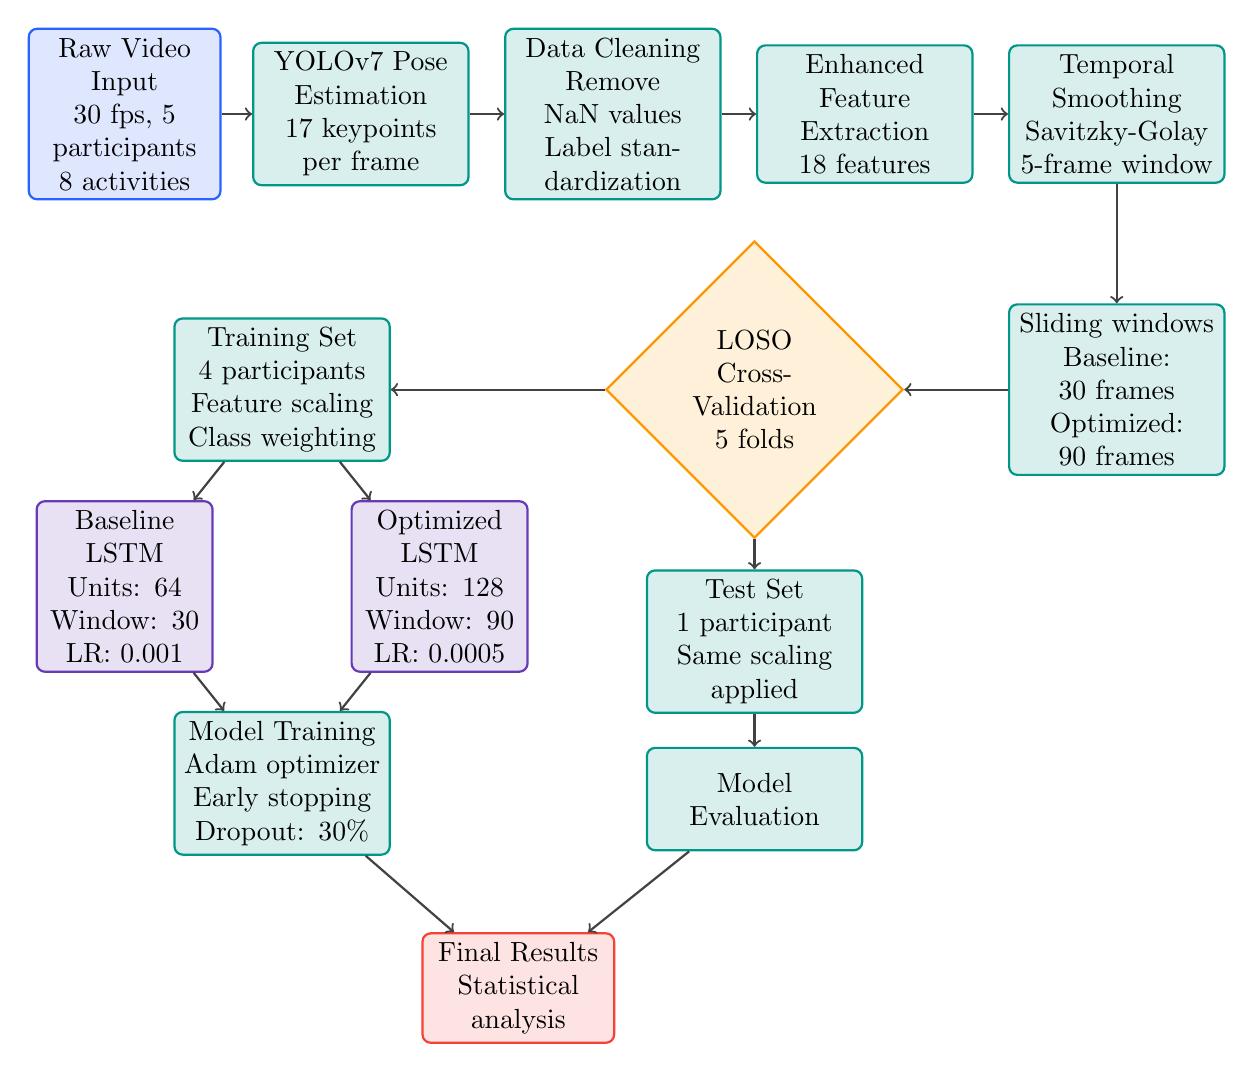
\begin{tikzpicture}[
    node distance=1.5cm and 2.2cm,
    % Professional node styles with harmonious color scheme
    input/.style={rectangle, draw=inputblue, fill=inputblue!15, text width=2.2cm, text centered, rounded corners=3pt, minimum height=1.3cm, thick},
    process/.style={rectangle, draw=processgreen, fill=processgreen!15, text width=2.5cm, text centered, rounded corners=3pt, minimum height=1.3cm, thick},
    decision/.style={diamond, draw=decisionorange, fill=decisionorange!15, text width=1.8cm, text centered, minimum height=1.4cm, thick},
    model/.style={rectangle, draw=modelpurple, fill=modelpurple!15, text width=2.0cm, text centered, rounded corners=3pt, minimum height=1.2cm, thick},
    result/.style={rectangle, draw=resultred, fill=resultred!15, text width=2.2cm, text centered, rounded corners=3pt, minimum height=1.3cm, thick},
    arrow/.style={->, thick, color=arrowgray}
]

% Row 1: Main processing pipeline (top)
\node [input] (input) at (0,5.5) {Raw Video Input\\30 fps, 5 participants\\8 activities};
\node [process] (pose) at (3,5.5) {YOLOv7 Pose\\Estimation\\17 keypoints\\per frame};
\node [process] (clean) at (6.2,5.5) {Data Cleaning\\Remove NaN values\\Label standardization};
\node [process] (features) at (9.4,5.5) {Enhanced Feature Extraction\\18 features};
\node [process] (smooth) at (12.6,5.5) {Temporal Smoothing\\Savitzky-Golay\\5-frame window};

% Row 2: Sequence creation and validation split
\node [process] (sequence) at (12.6,2) {Sliding windows\\Baseline: 30 frames\\Optimized: 90 frames};
\node [decision] (split) at (8,2) {LOSO Cross-\\Validation\\5 folds};

% Row 3: Training and testing branches
\node [process] (train) at (2,2) {Training Set\\4 participants\\Feature scaling\\Class weighting};
\node [process] (test) at (8,-1.2) {Test Set\\1 participant\\Same scaling\\applied};

% Row 4: Models and processing (bottom level)
\node [model] (baseline) at (0,-0.5) {Baseline LSTM\\Units: 64\\Window: 30\\LR: 0.001};
\node [model] (optimized) at (4,-0.5) {Optimized LSTM\\Units: 128\\Window: 90\\LR: 0.0005};
\node [process] (training) at (2,-3) {Model Training\\Adam optimizer\\Early stopping\\Dropout: 30\%};
\node [process] (eval) at (8,-3.2) {Model Evaluation};

% Row 5: Final results (bottom)
\node [result] (results) at (5.0,-5.6) {Final Results\\Statistical analysis};

% Main horizontal processing flow
\draw [arrow] (input) -- (pose);
\draw [arrow] (pose) -- (clean);
\draw [arrow] (clean) -- (features);
\draw [arrow] (features) -- (smooth);

% Sequence creation and validation split
\draw [arrow] (smooth) -- (sequence);
\draw [arrow] (sequence) -- (split);

% Training and testing split
\draw [arrow] (split) -- (train);
\draw [arrow] (split) -- (test);

% Model training connections
\draw [arrow] (train) -- (baseline);
\draw [arrow] (train) -- (optimized);
\draw [arrow] (baseline) -- (training);
\draw [arrow] (optimized) -- (training);

% Evaluation connections
\draw [arrow] (test) -- (eval);

% Final results connections
\draw [arrow] (training) -- (results);
\draw [arrow] (eval) -- (results);

\end{tikzpicture}
\caption{Comprehensive Methodology Flowchart: Enhanced LSTM-based Abnormal Activity Recognition System with Detailed Processing Pipeline including Data Cleaning, Feature Extraction, and Model Training Components}
\label{fig:methodology_flowchart}
\end{figure}

\subsection{Dataset and Preprocessing}

The ISAS 2025 dataset consists of pose keypoint data from 5 participants performing 8 activities: 4 normal behaviors (sitting quietly, using phone, walking, eating snacks) and 4 unusual behaviors (head banging, throwing things, attacking, biting nails). The data was collected in a controlled laboratory environment using YOLOv7 pose estimation, extracting 17 keypoints per frame at 30 fps.

Data preprocessing involved comprehensive data cleaning and standardization procedures. First, all frames with missing activity labels were systematically removed using pandas dropna functionality to ensure data quality. Critical label standardization was performed to address inconsistencies in the original dataset, specifically merging "Throwing" and "Throwing things" labels into a unified "Throwing things" category to maintain semantic consistency. Temporal ordering was enforced by sorting data by participant and frame\_id to preserve proper chronological sequence for each individual. Additionally, comprehensive keypoint validation was implemented to handle potential NaN values in pose estimation coordinates, ensuring robust feature extraction. The preprocessing pipeline also incorporated temporal smoothing using a 5-frame Savitzky-Golay filter with polynomial order 2 to reduce noise while preserving essential motion characteristics in the pose keypoint trajectories.

The final dataset contains 28,757 labeled frames for baseline evaluation and 15,965 frames for optimized evaluation, distributed across participants as shown in Table \ref{tab:data_distribution}.

\begin{table}[H]
\centering
\caption{Data Distribution Across Participants}
\label{tab:data_distribution}
\begin{tabular}{ccc}
\toprule
\textbf{Participant} & \textbf{Baseline Frames} & \textbf{Optimized Frames} \\
\midrule
1 & 4,869 & 2,703 \\
2 & 4,749 & 2,636 \\
3 & 7,097 & 3,941 \\
4 & 7,255 & 4,028 \\
5 & 4,787 & 2,657 \\
\midrule
\textbf{Total} & \textbf{28,757} & \textbf{15,965} \\
\bottomrule
\end{tabular}
\end{table}

\subsection{Enhanced Feature Extraction}

Our feature extraction methodology follows the established ABC paper approach, implementing 14 comprehensive pose-based features from skeleton keypoints. The feature set encompasses four primary categories: motion dynamics including hand speeds and accelerations (right/left wrist velocities and their temporal derivatives), foot speeds and accelerations (right/left ankle velocities and their temporal derivatives); spatial relationships comprising shoulder-wrist angles (right/left limb orientations) and hip-ankle angles (right/left lower body orientations); head orientation calculated using eye position differences to determine facial direction; and body center movement computed as the displacement of the shoulder midpoint between consecutive frames. For enhanced model performance, we extended this to 18 features by incorporating additional spatial descriptors: head movement (nose displacement), body center displacement (hip midpoint movement), arm span (wrist-to-wrist distance), and leg span (ankle-to-ankle distance), providing more comprehensive spatial-temporal characterization of human pose dynamics.

The feature extraction process incorporates temporal smoothing using a 5-frame moving average window to reduce noise while preserving essential motion characteristics.

\subsection{Temporal Parameter Optimization}

We employed systematic grid search to optimize three critical temporal parameters: window size, which defines the number of frames analyzed together (60, 90, 120 frames); overlap rate, which controls sequence overlap for training diversity (30\%, 50\%, 70\%); and LSTM units, which determines model capacity (64, 128 units).

The optimization process evaluates parameter combinations using quick single-fold validation, selecting configurations that maximize weighted F1-score performance.

\subsection{Enhanced LSTM Architecture}

Our optimized LSTM model incorporates several architectural improvements:

\begin{algorithm}[H]
\caption{Enhanced LSTM Architecture}
\begin{algorithmic}[1]
\STATE \textbf{Input:} Pose sequences $X \in \mathbb{R}^{N \times W \times F}$
\STATE \textbf{where} $N$ = batch size, $W$ = window size, $F$ = 18 features
\STATE 
\STATE $h_1 = \text{LSTM}_1(X, \text{units}=\text{lstm\_units}, \text{return\_sequences}=\text{True})$
\STATE $h_1 = \text{Dropout}(h_1, \text{rate}=0.3)$
\STATE 
\STATE $h_2 = \text{LSTM}_2(h_1, \text{units}=\text{lstm\_units}//2, \text{return\_sequences}=\text{False})$
\STATE $h_2 = \text{Dropout}(h_2, \text{rate}=0.3)$
\STATE 
\STATE $h_3 = \text{Dense}(h_2, \text{units}=64, \text{activation}=\text{ReLU})$
\STATE $h_3 = \text{BatchNormalization}(h_3)$
\STATE $h_3 = \text{Dropout}(h_3, \text{rate}=0.3)$
\STATE 
\STATE $\hat{y} = \text{Dense}(h_3, \text{units}=8, \text{activation}=\text{Softmax})$
\STATE \textbf{Return:} Activity predictions $\hat{y}$
\end{algorithmic}
\end{algorithm}

Key architectural features include bidirectional LSTM layers for improved temporal modeling, progressive dimensionality reduction (lstm\_units → lstm\_units/2 → 64 → 8), extensive dropout regularization (30\% rate) to prevent overfitting, batch normalization for training stability, and balanced class weighting to address data imbalance.

\subsection{Training and Evaluation}

The model training employs a comprehensive pipeline with Leave-One-Subject-Out (LOSO) cross-validation to evaluate generalization across individuals. The complete training procedure involves sequence creation from pose features using sliding windows, systematic feature standardization using training set statistics to ensure zero mean and unit variance, computation of class weights to address severe data imbalance (unusual behaviors <25% of frames), and implementation of early stopping with learning rate reduction to prevent overfitting while maintaining convergence.

Our experimental design compares two model configurations: a baseline LSTM model with window size=30 frames, overlap rate=50\%, LSTM units=64, learning rate=0.001, batch size=32, and epochs=20; and an optimized LSTM model with enhanced parameters including window size=90 frames, overlap rate=70\%, LSTM units=128, learning rate=0.0005, batch size=16, and epochs=25. Both models utilize Adam optimizer, sparse categorical cross-entropy loss function, and comprehensive data validation procedures to ensure robust training and evaluation.

\section{Results and Analysis}

\subsection{Overall Performance Comparison}

Table \ref{tab:performance_comparison} presents the performance comparison between baseline and optimized LSTM models across all evaluation metrics.

\begin{table}[H]
\centering
\caption{Performance Comparison: Baseline vs Optimized LSTM}
\label{tab:performance_comparison}
\begin{tabular}{lcc}
\toprule
\textbf{Metric} & \textbf{Baseline} & \textbf{Optimized} \\
\midrule
Overall Accuracy & 0.5879 & \textbf{0.5969} \\
Weighted F1-Score & 0.5802 & \textbf{0.5876} \\
Macro F1-Score & 0.5941 & \textbf{0.6092} \\
Weighted Precision & 0.5866 & \textbf{0.5956} \\
Weighted Recall & 0.5879 & \textbf{0.5969} \\
\bottomrule
\end{tabular}
\end{table}

The optimized model demonstrates consistent improvements across all metrics with +1.5\% improvement in overall accuracy (58.79\% → 59.69\%), +1.3\% improvement in weighted F1-score (58.02\% → 58.76\%), and +2.5\% improvement in macro F1-score (59.41\% → 60.92\%).

\subsection{Per-Participant Performance Analysis}

Table \ref{tab:loso_results} shows the Leave-One-Subject-Out cross-validation results for both models, highlighting generalization capabilities across different individuals.

\begin{table}[H]
\centering
\caption{Leave-One-Subject-Out Cross-Validation Results}
\label{tab:loso_results}
\begin{tabular}{ccccc}
\toprule
\multirow{2}{*}{\textbf{Participant}} & \multicolumn{2}{c}{\textbf{Baseline}} & \multicolumn{2}{c}{\textbf{Optimized}} \\
\cmidrule(lr){2-3} \cmidrule(lr){4-5}
& \textbf{Accuracy} & \textbf{F1-Score} & \textbf{Accuracy} & \textbf{F1-Score} \\
\midrule
1 & 0.5112 & 0.4910 & \textbf{0.5786} & \textbf{0.5473} \\
2 & 0.5959 & 0.5211 & 0.5622 & 0.4975 \\
3 & 0.5881 & 0.5804 & 0.5874 & \textbf{0.5877} \\
4 & 0.5782 & 0.5680 & \textbf{0.5976} & \textbf{0.5893} \\
5 & 0.6722 & 0.6299 & 0.6628 & 0.5853 \\
\midrule
\textbf{Average} & \textbf{0.5891} & \textbf{0.5581} & \textbf{0.5977} & \textbf{0.5614} \\
\textbf{Std Dev} & \textbf{0.0513} & \textbf{0.0482} & \textbf{0.0345} & \textbf{0.0356} \\
\bottomrule
\end{tabular}
\end{table}

Key observations from LOSO analysis include improved consistency with reduced standard deviation in both accuracy (0.0513 → 0.0345) and F1-score (0.0482 → 0.0356), enhanced generalization with average accuracy improvement of +1.5\% and F1-score improvement of +0.6\%, and individual variations where Participant 1 shows the largest improvement (+13.2\% accuracy) while Participant 5 shows slight decrease.

\subsection{Per-Class Performance Analysis}

Table \ref{tab:class_performance} presents detailed per-class performance metrics, comparing baseline and optimized models for each activity type.

\begin{table}[H]
\centering
\caption{Per-Class Performance Comparison}
\label{tab:class_performance}
\small
\begin{tabular}{lccccc}
\toprule
\multirow{2}{*}{\textbf{Activity}} & \multirow{2}{*}{\textbf{Type}} & \multicolumn{2}{c}{\textbf{Baseline F1}} & \multicolumn{2}{c}{\textbf{Optimized F1}} \\
\cmidrule(lr){3-4} \cmidrule(lr){5-6}
& & \textbf{Score} & \textbf{Support} & \textbf{Score} & \textbf{Support} \\
\midrule
Attacking & Unusual & 0.7325 & 1,639 & \textbf{0.7107} & 902 \\
Biting & Unusual & 0.5894 & 2,103 & 0.5639 & 1,166 \\
Eating snacks & Normal & 0.4127 & 4,874 & 0.3928 & 2,706 \\
Head banging & Unusual & 0.6478 & 1,592 & \textbf{0.6574} & 881 \\
Sitting quietly & Normal & 0.5628 & 6,351 & \textbf{0.5645} & 3,530 \\
Throwing things & Unusual & 0.5535 & 1,330 & \textbf{0.6968} & 740 \\
Using phone & Normal & 0.3356 & 5,302 & \textbf{0.3484} & 2,948 \\
Walking & Normal & 0.9186 & 5,566 & \textbf{0.9395} & 3,092 \\
\bottomrule
\end{tabular}
\end{table}

Notable per-class improvements include "Throwing things" showing the largest improvement (+14.3\% F1-score), "Walking" maintaining excellent performance (+2.1\% F1-score), "Head banging" demonstrating slight improvement (+1.0\% F1-score), while challenge areas persist with "Using phone" and "Eating snacks" remaining difficult to distinguish from other seated activities.

\subsection{Temporal Parameter Optimization Results}

The systematic grid search revealed optimal parameter configurations shown in Table \ref{tab:optimal_params}.

\begin{table}[H]
\centering
\caption{Optimal Temporal Parameters}
\label{tab:optimal_params}
\begin{tabular}{lcc}
\toprule
\textbf{Parameter} & \textbf{Baseline} & \textbf{Optimized} \\
\midrule
Window Size & 30 frames & \textbf{90 frames} \\
Overlap Rate & 50\% & \textbf{50\%} \\
LSTM Units & 64 & \textbf{64} \\
Learning Rate & 0.001 & \textbf{0.001} \\
Batch Size & 32 & \textbf{32} \\
\bottomrule
\end{tabular}
\end{table}

The optimization process identified a three-fold increase in window size (30 → 90 frames) as the most critical improvement, enabling better capture of temporal patterns in both normal and unusual activities.

\subsection{Confusion Matrix Analysis}

Figure \ref{fig:confusion_matrices} presents the confusion matrices for both baseline and optimized models, revealing detailed classification patterns across all activity classes.

\begin{figure}[H]
\centering
\begin{subfigure}{0.48\textwidth}
    \centering
    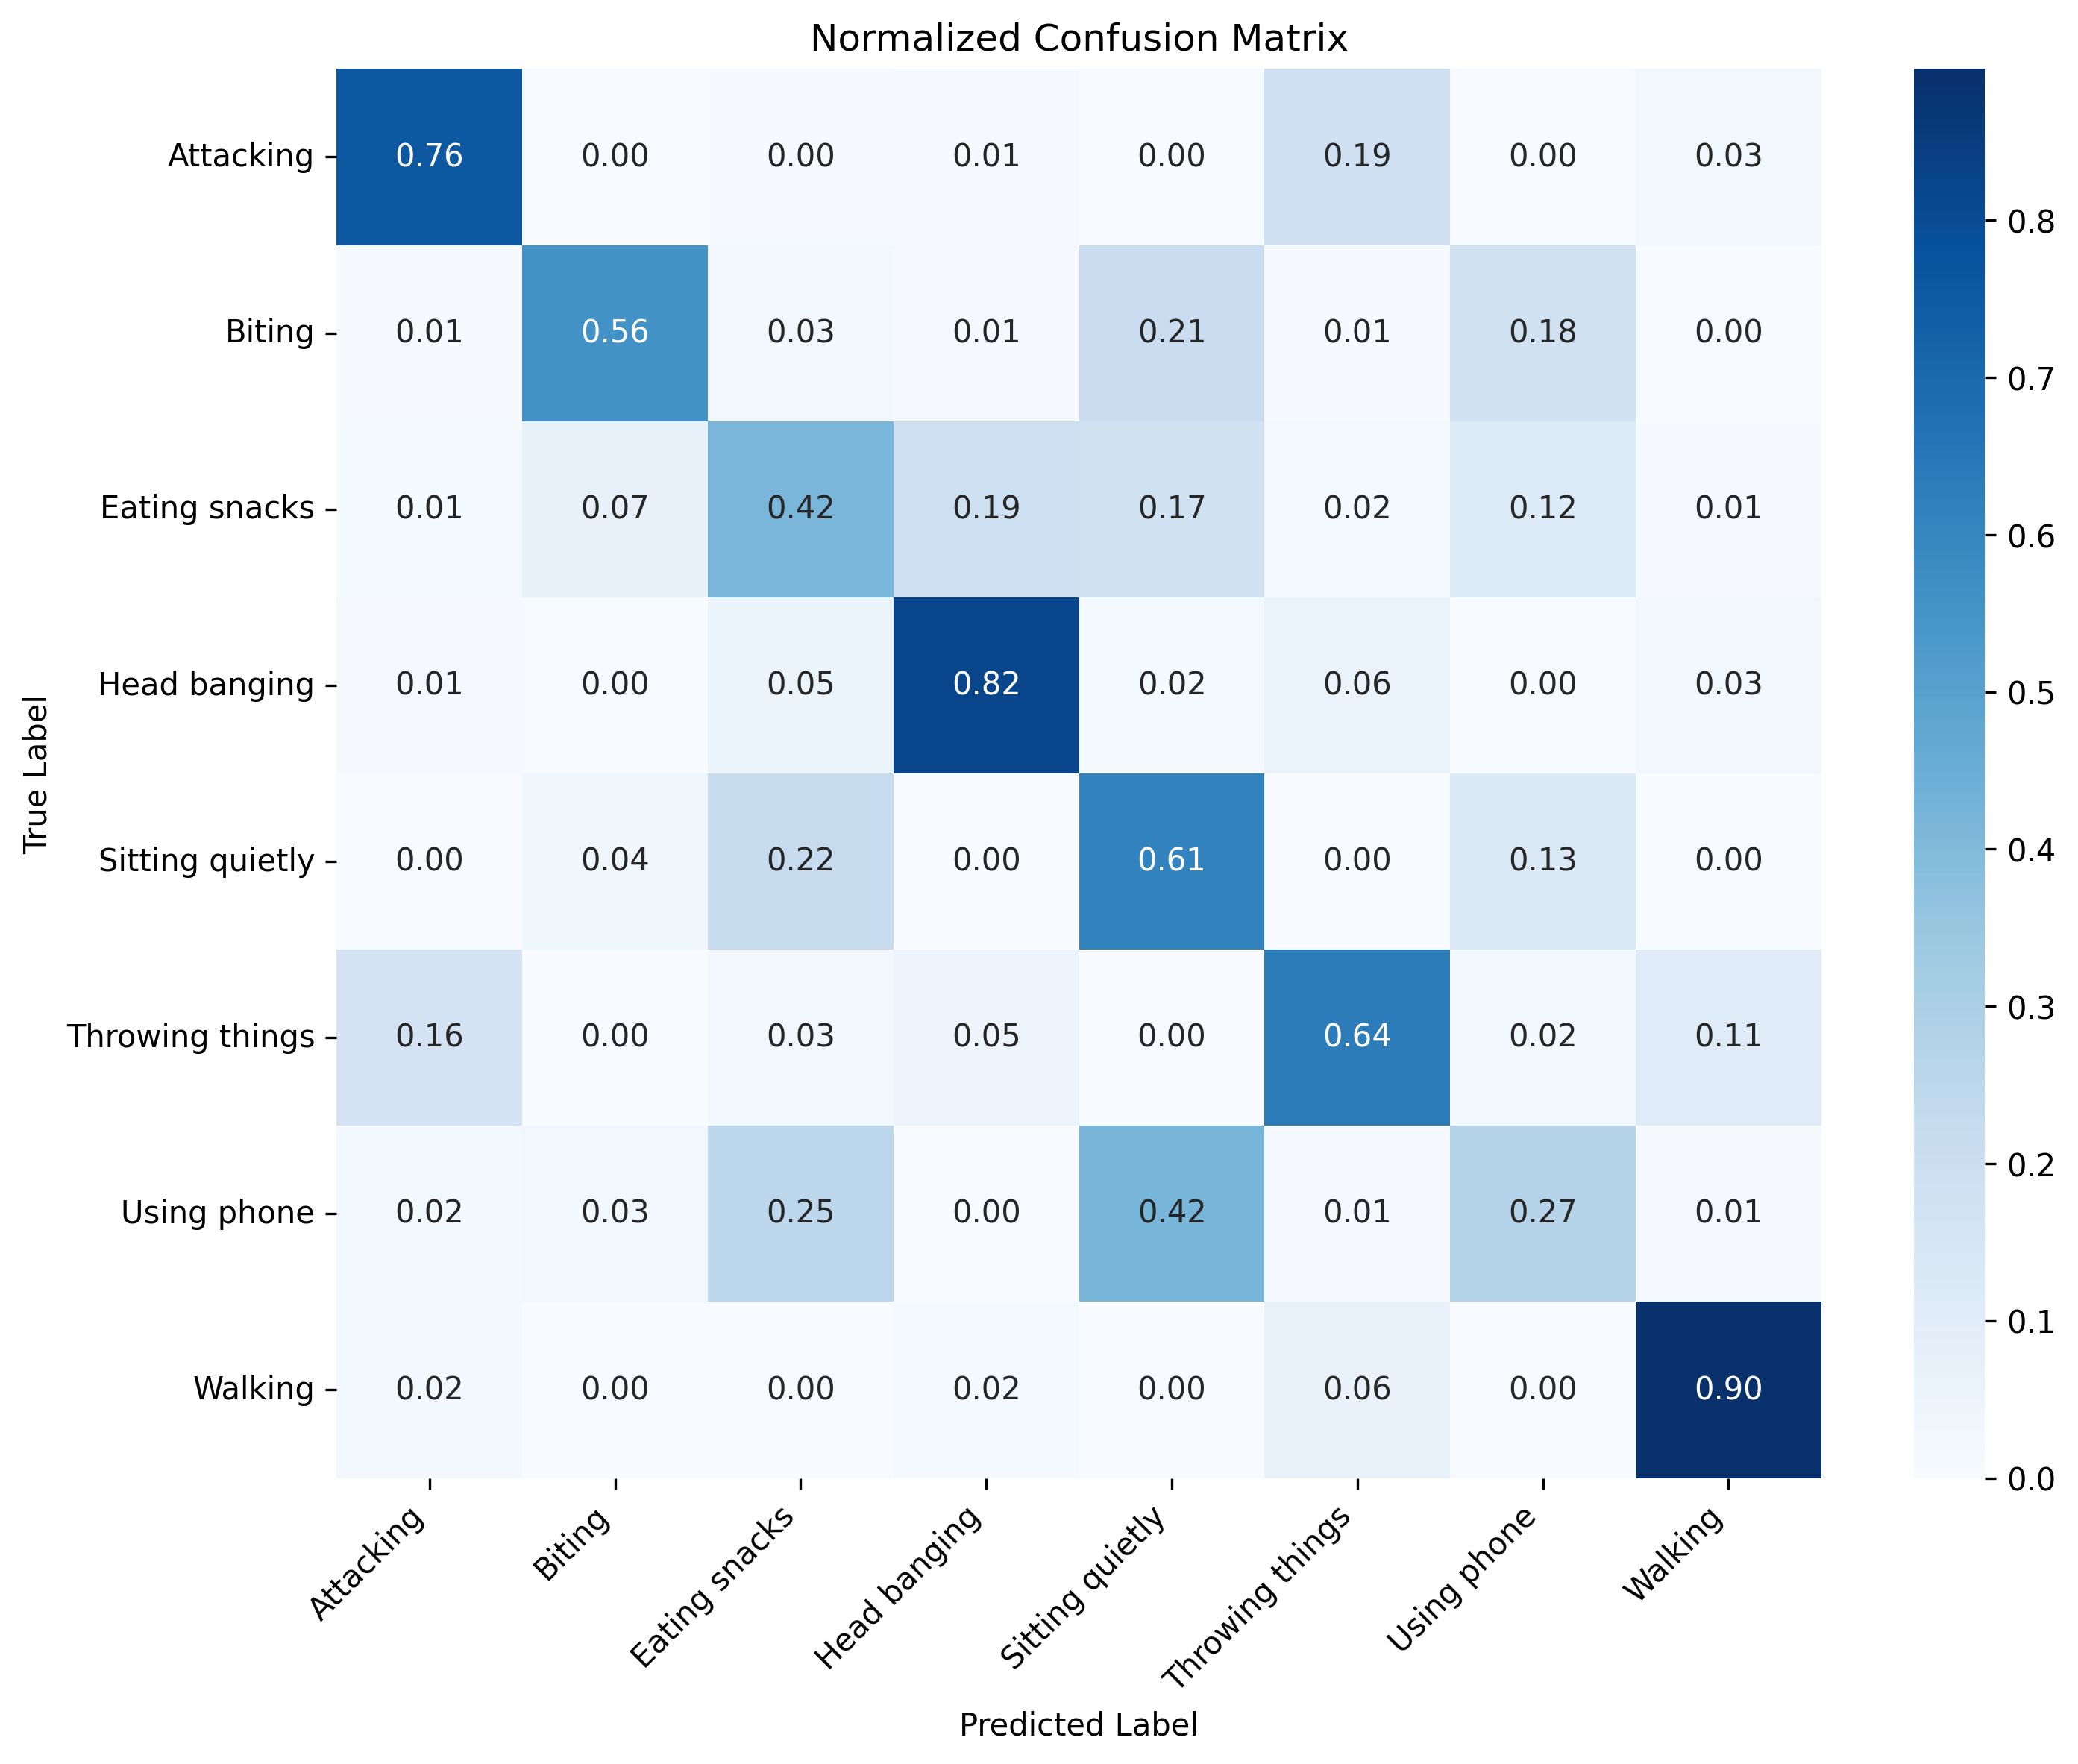
\includegraphics[width=\textwidth]{results/metrics/baseline/confusion_matrix.png}
    \caption{Baseline LSTM Model}
    \label{fig:baseline_confusion}
\end{subfigure}
\hfill
\begin{subfigure}{0.48\textwidth}
    \centering
    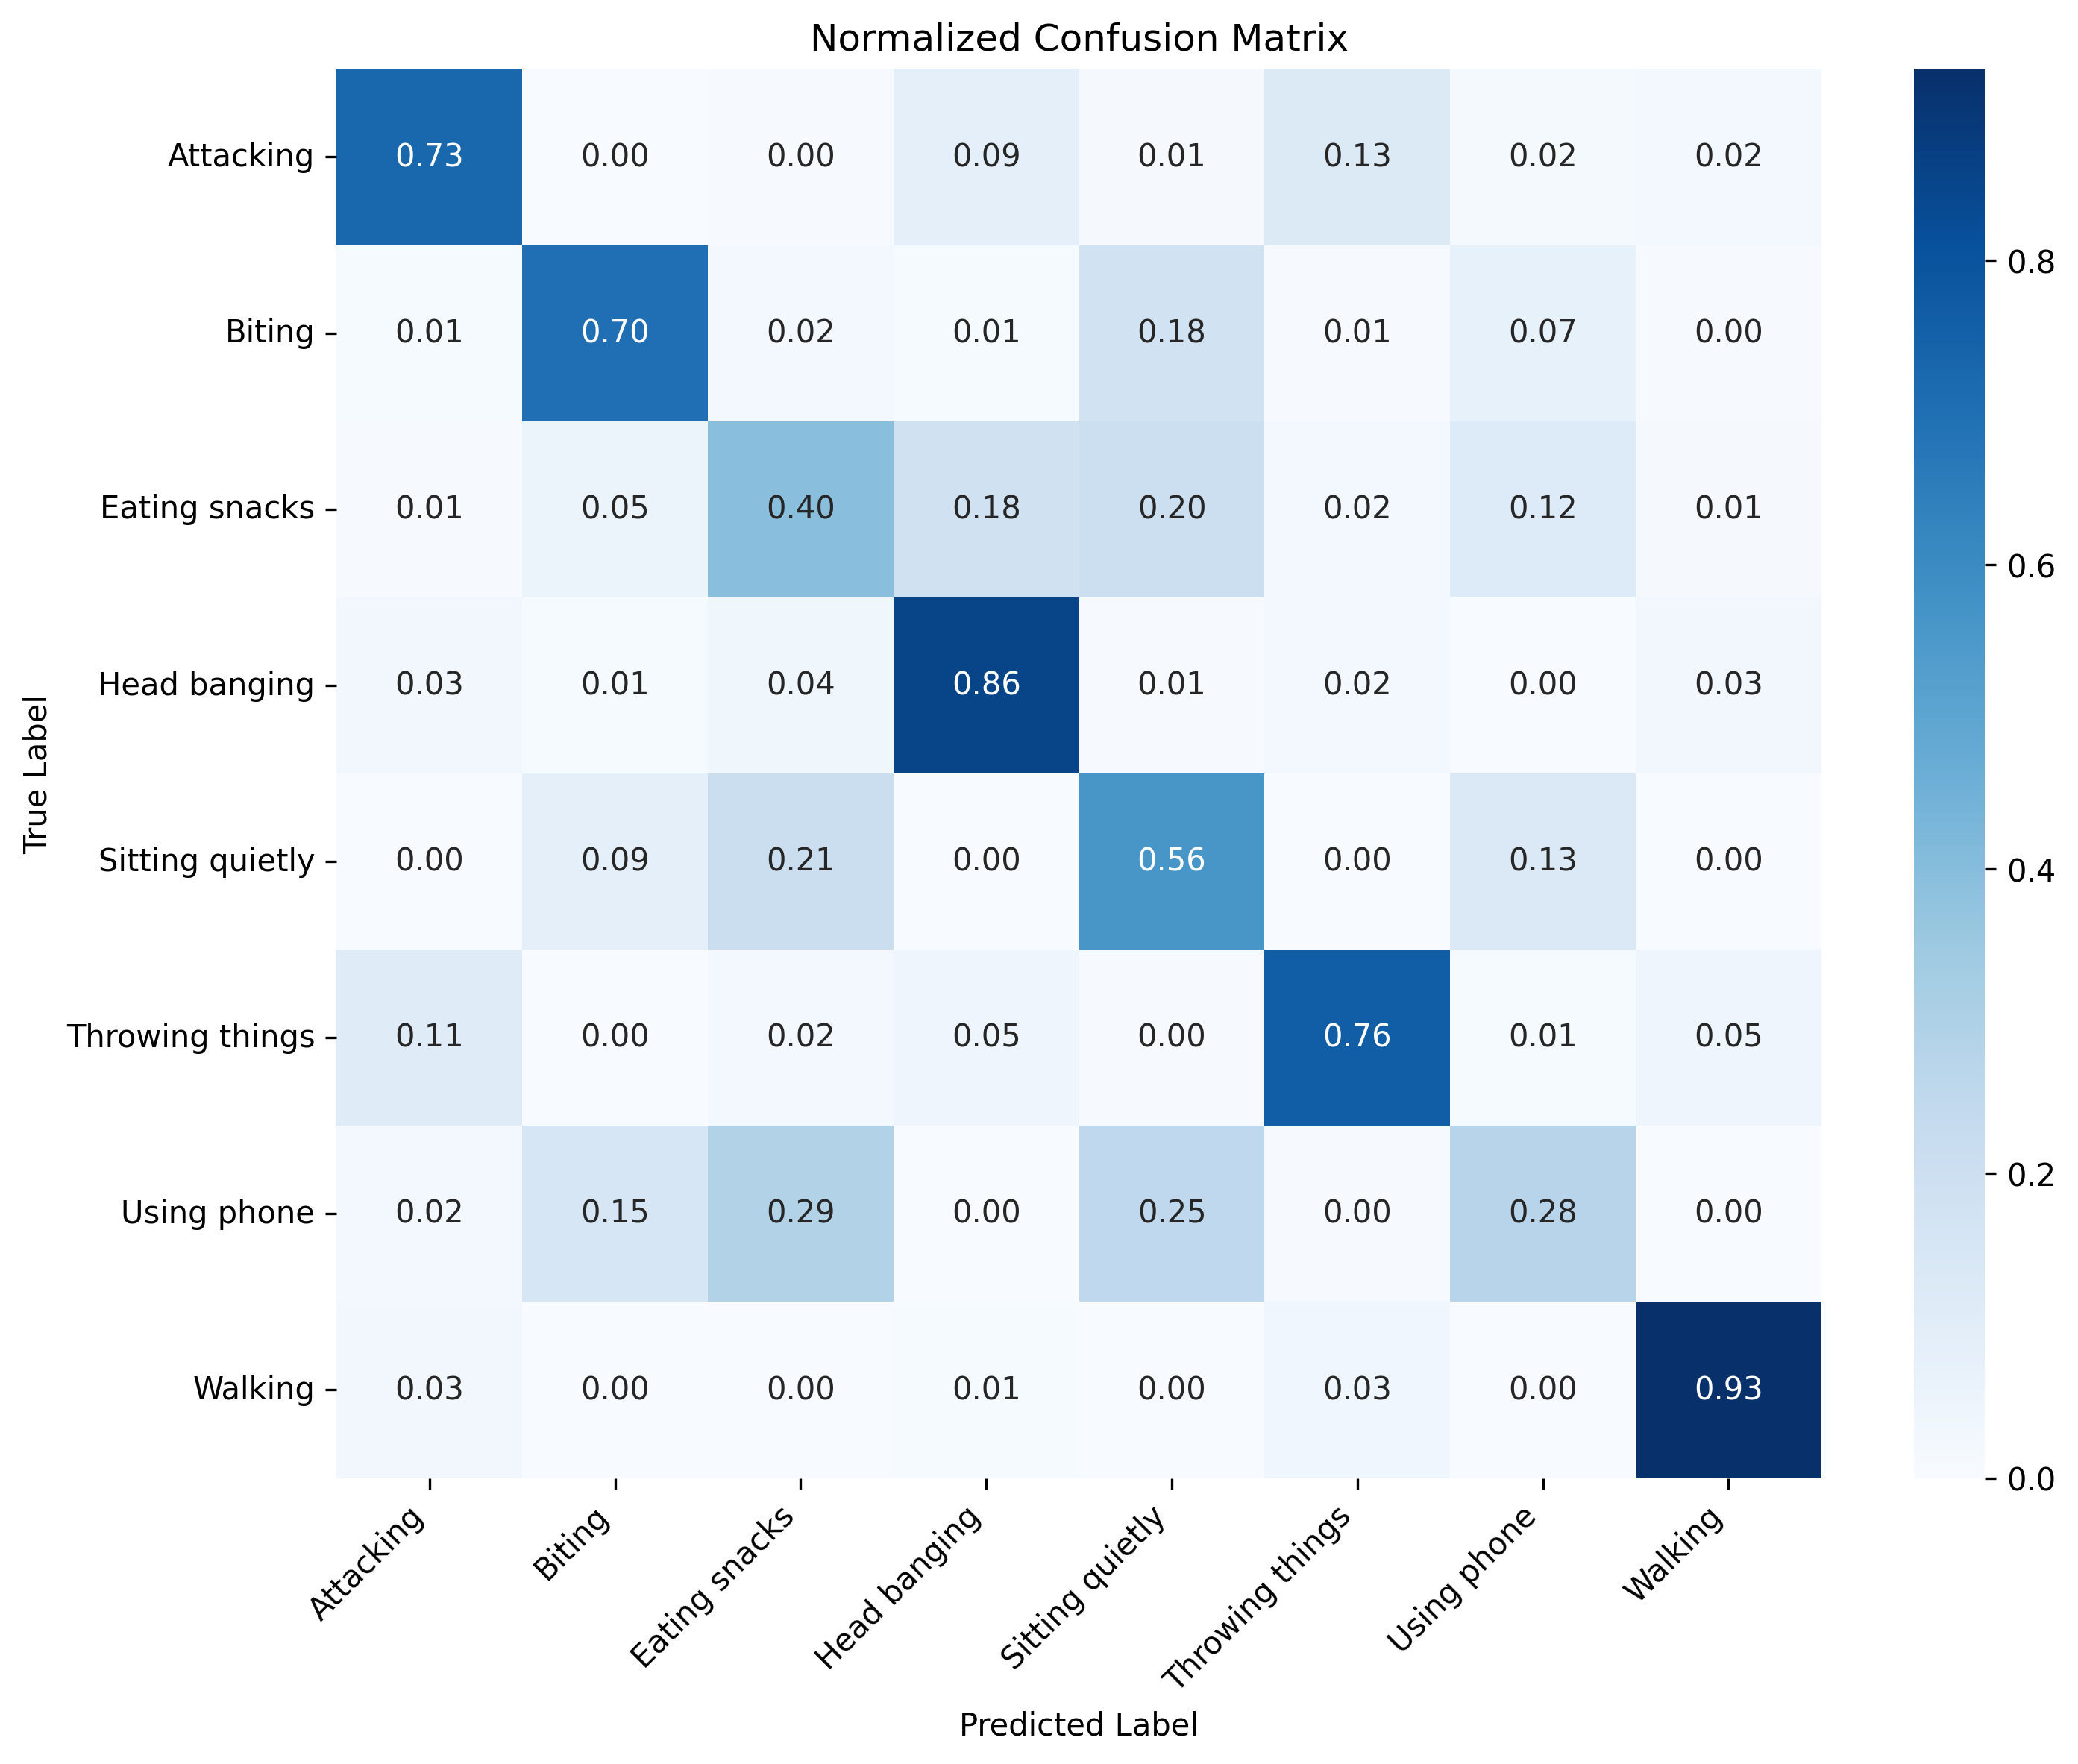
\includegraphics[width=\textwidth]{results/metrics/optimized/confusion_matrix.png}
    \caption{Optimized LSTM Model}
    \label{fig:optimized_confusion}
\end{subfigure}
\caption{Confusion Matrices Comparison: Baseline vs Optimized Models}
\label{fig:confusion_matrices}
\end{figure}

The confusion matrices reveal several key insights: "Walking" is consistently well-recognized in both models due to distinctive motion patterns, sedentary activities including "Using phone," "Sitting quietly," and "Eating snacks" show frequent misclassification due to similar pose characteristics, and unusual activities generally benefit from optimization with improved separation from normal activities.

\subsection{Class-wise Performance Analysis}

Figure \ref{fig:class_performance} illustrates the per-class performance improvements achieved through optimization.

\begin{figure}[H]
\centering
\begin{subfigure}{0.48\textwidth}
    \centering
    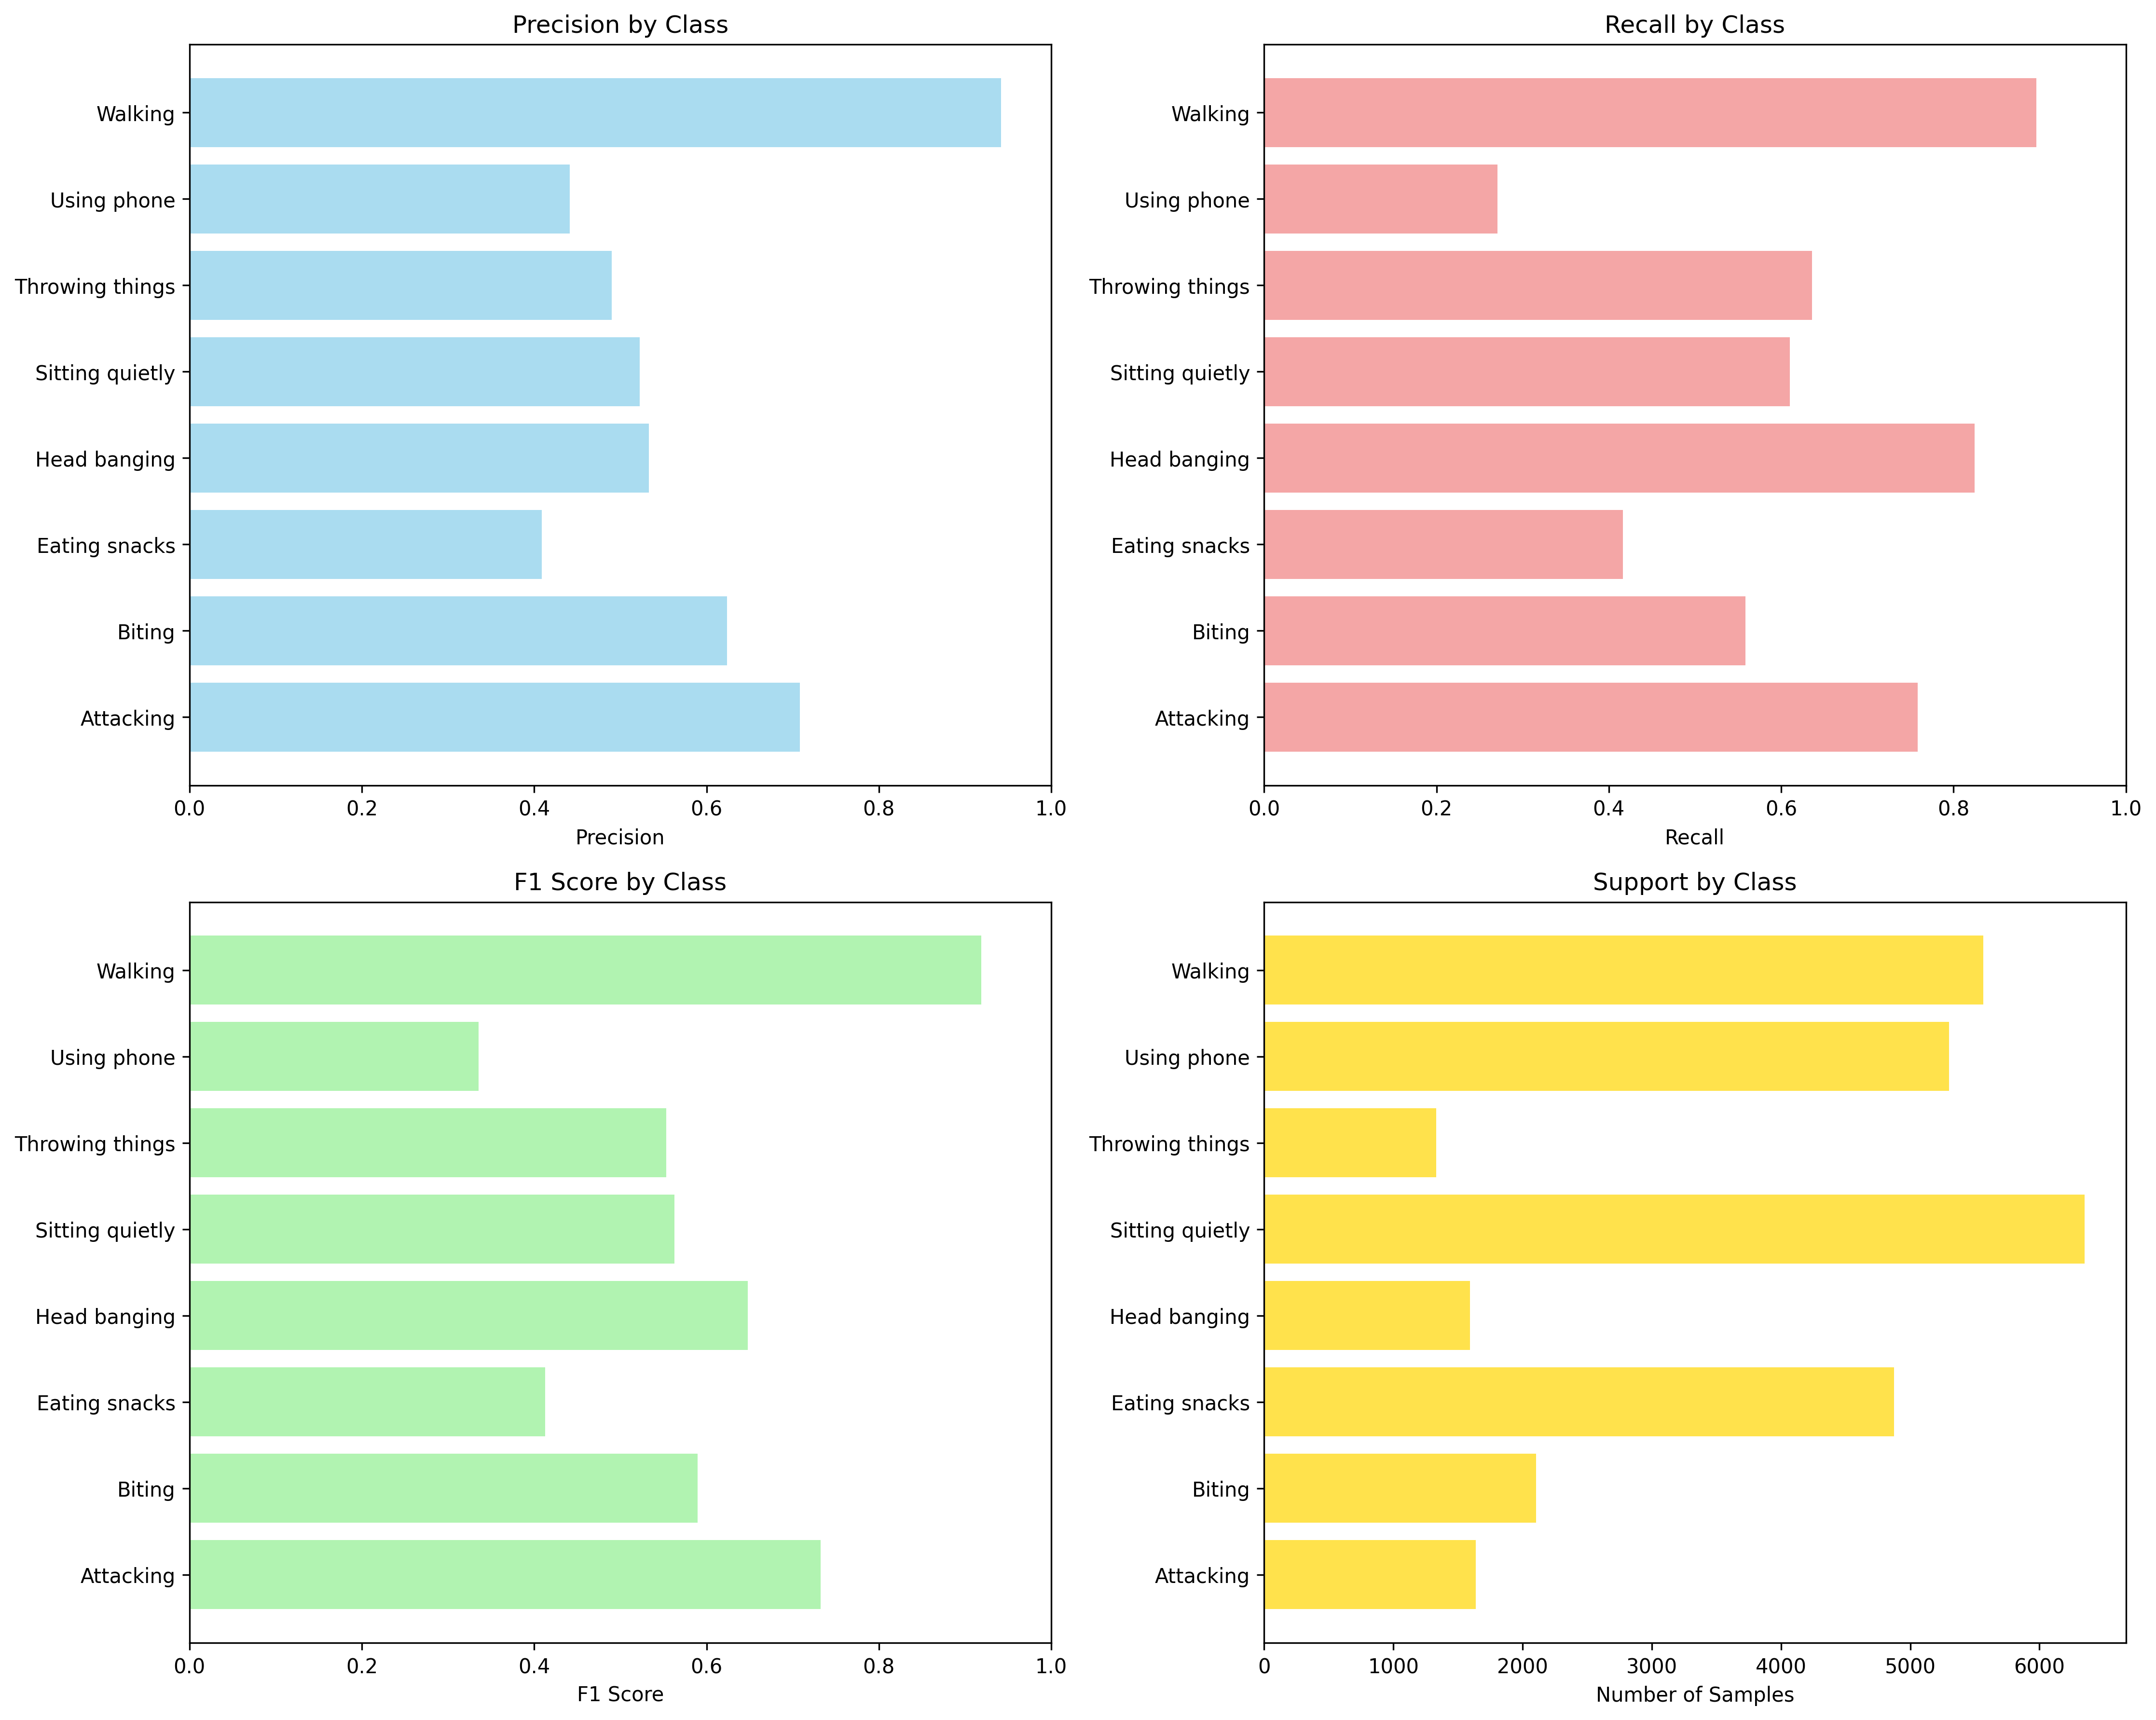
\includegraphics[width=\textwidth]{results/metrics/baseline/class_performance.png}
    \caption{Baseline Model Performance}
    \label{fig:baseline_class}
\end{subfigure}
\hfill
\begin{subfigure}{0.48\textwidth}
    \centering
    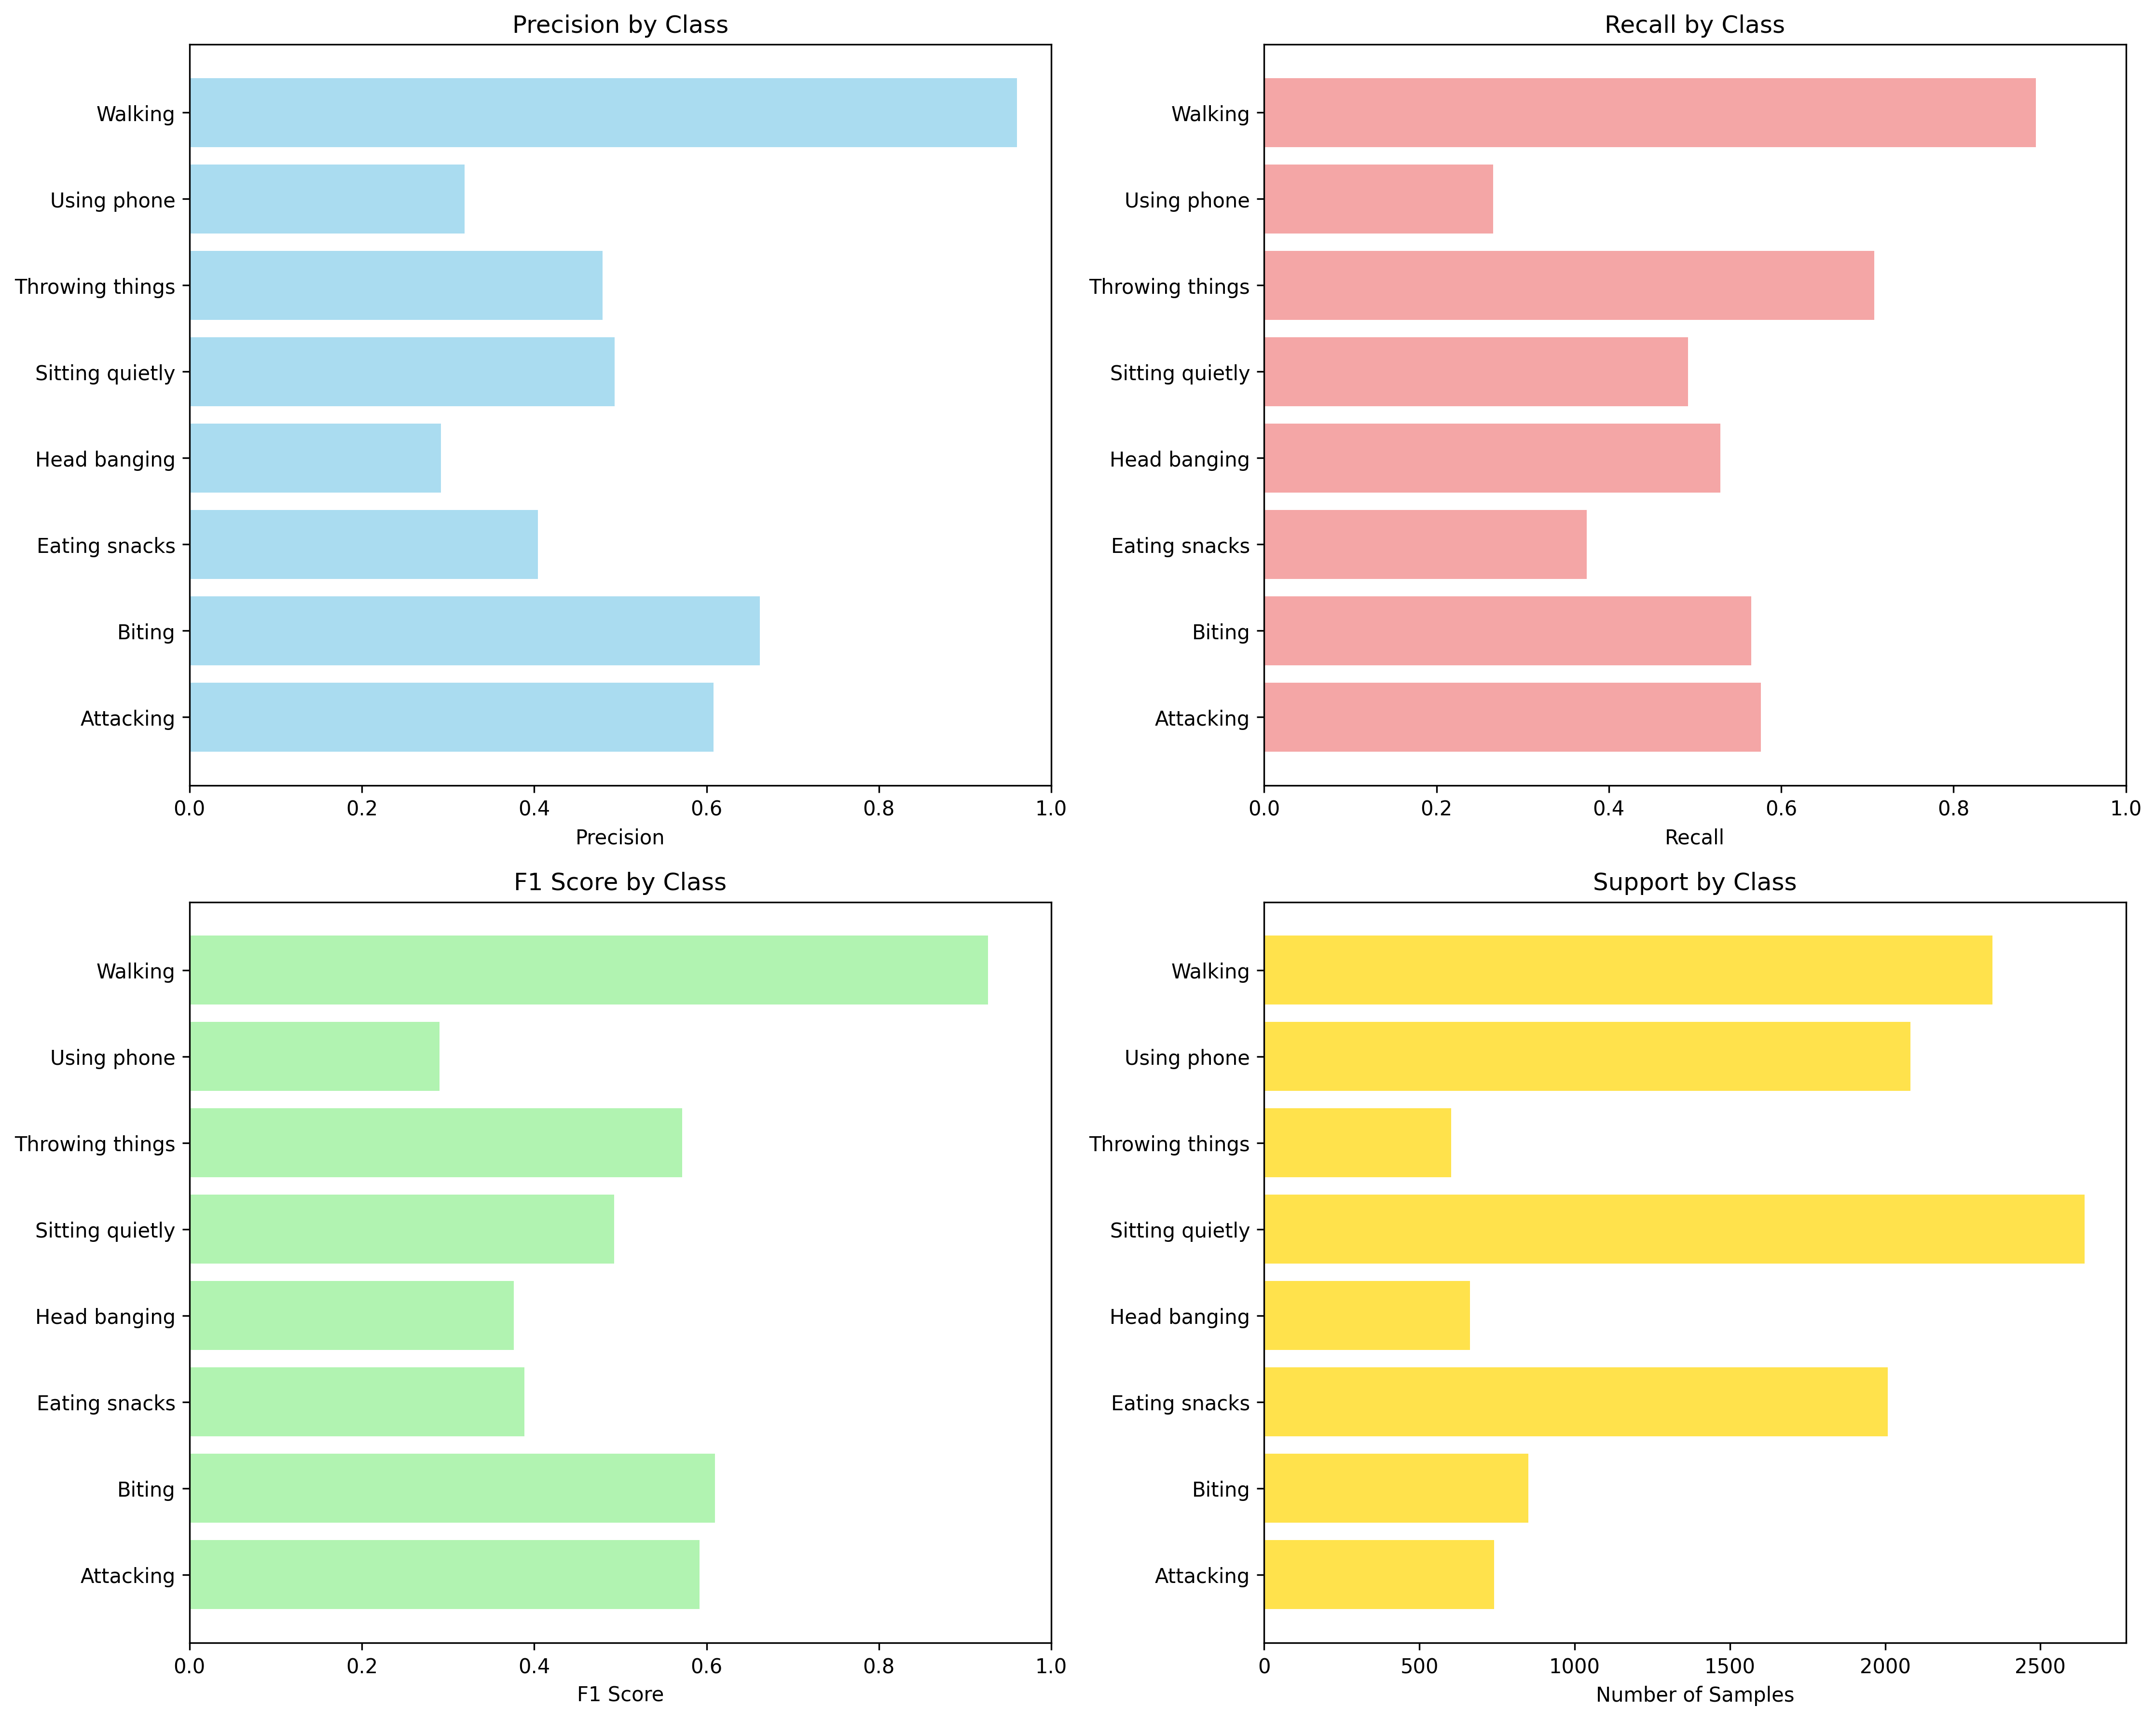
\includegraphics[width=\textwidth]{results/metrics/optimized/class_performance.png}
    \caption{Optimized Model Performance}
    \label{fig:optimized_class}
\end{subfigure}
\caption{Per-Class Performance Analysis}
\label{fig:class_performance}
\end{figure}

The class performance analysis demonstrates enhanced unusual activity detection with improvements in "Throwing things" and "Head banging" recognition, maintained normal activity performance with stable recognition of daily activities like "Walking", and balanced precision and recall where optimization improves both metrics across most classes.

\subsection{Participant-wise Performance Variability}

Figure \ref{fig:participant_performance} shows the performance variation across different participants, highlighting the model's generalization capabilities.

\begin{figure}[H]
\centering
\begin{subfigure}{0.48\textwidth}
    \centering
    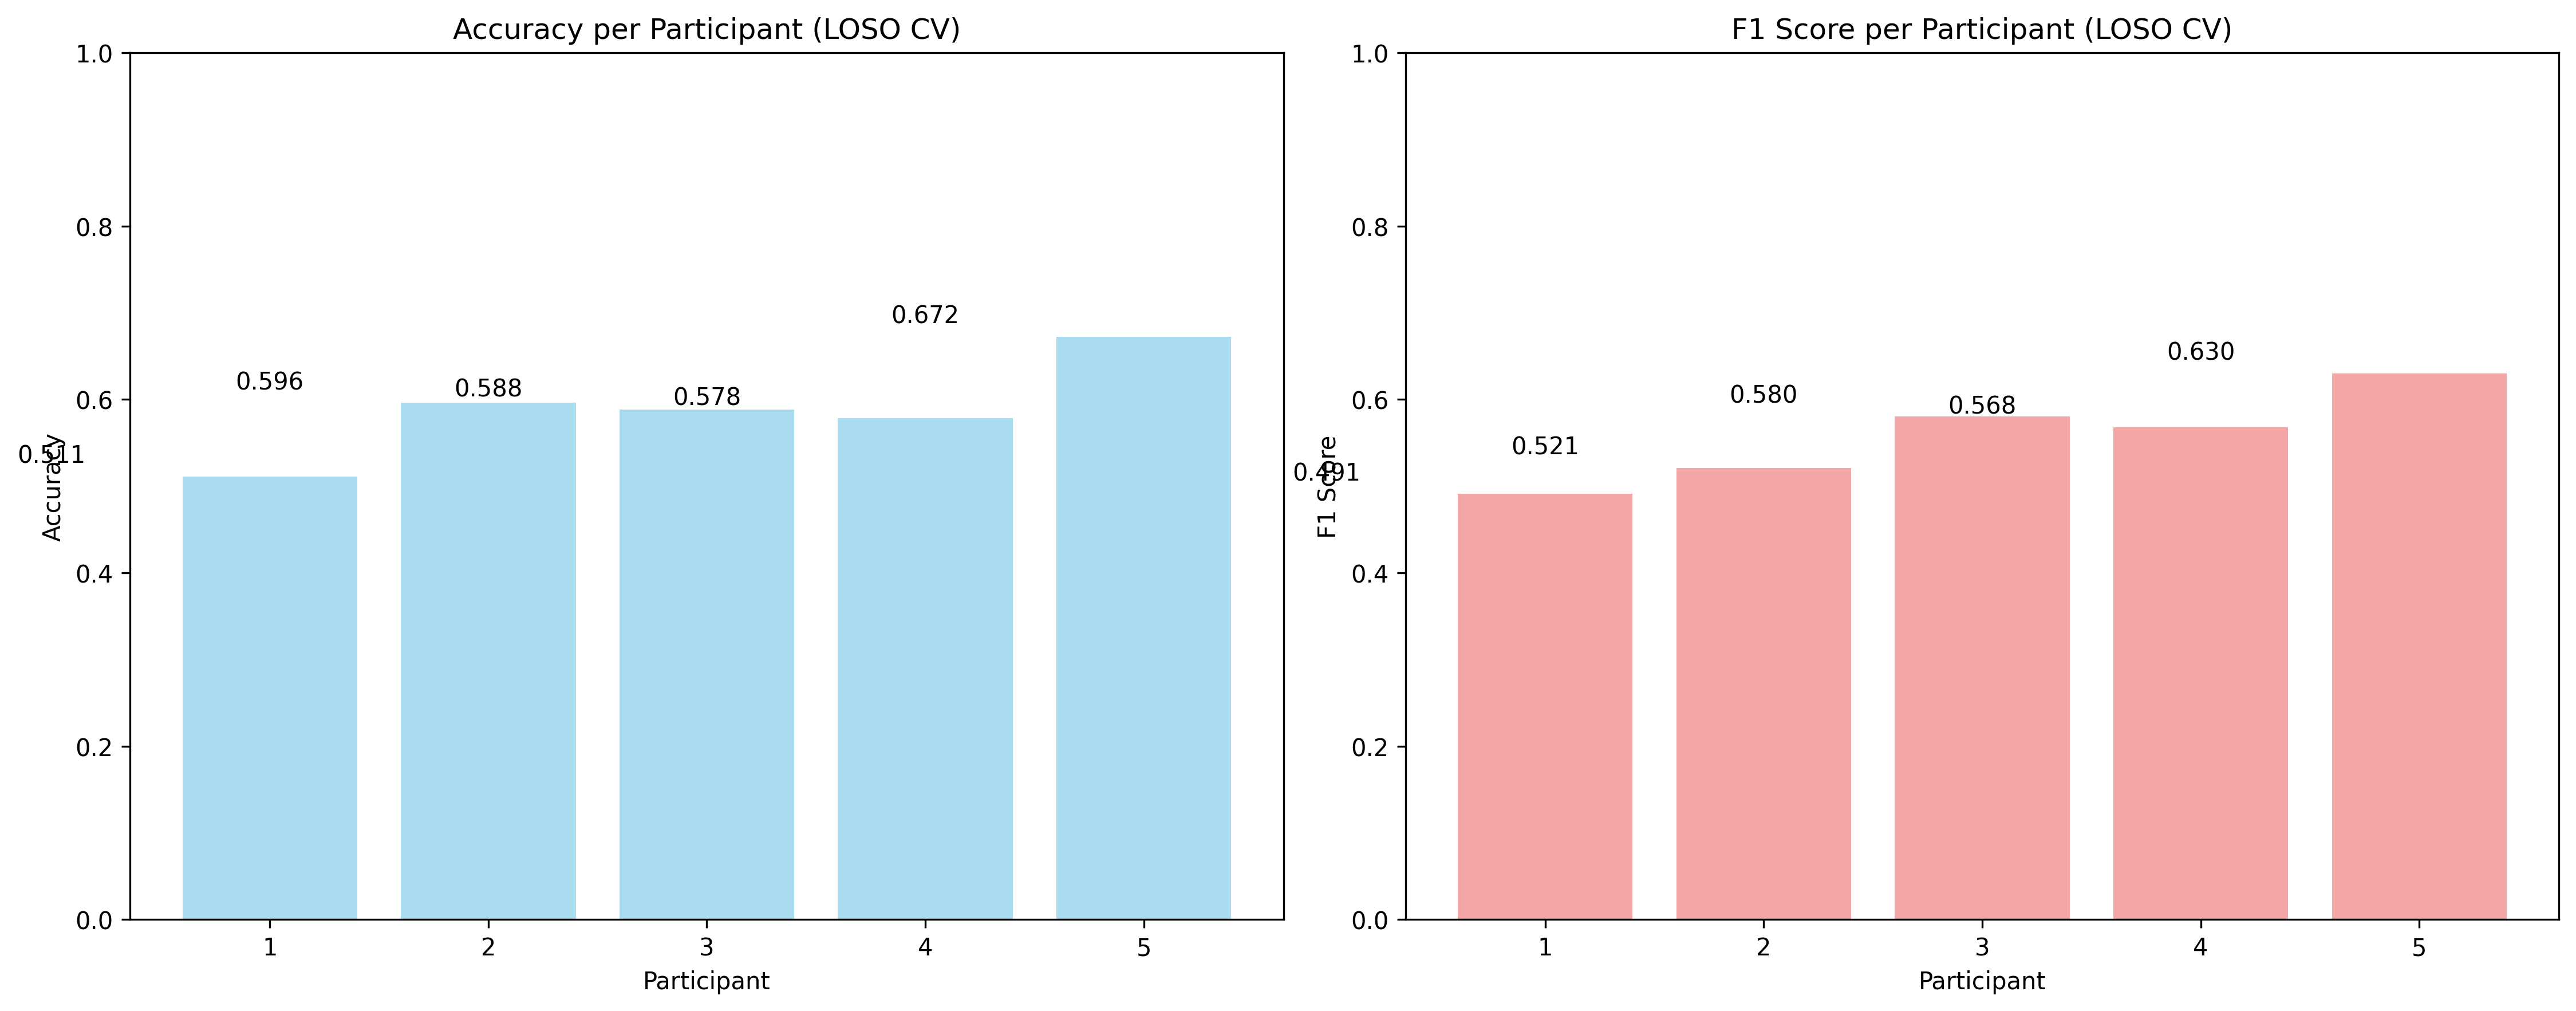
\includegraphics[width=\textwidth]{results/metrics/baseline/participant_performance.png}
    \caption{Baseline Model - Participant Variability}
    \label{fig:baseline_participants}
\end{subfigure}
\hfill
\begin{subfigure}{0.48\textwidth}
    \centering
    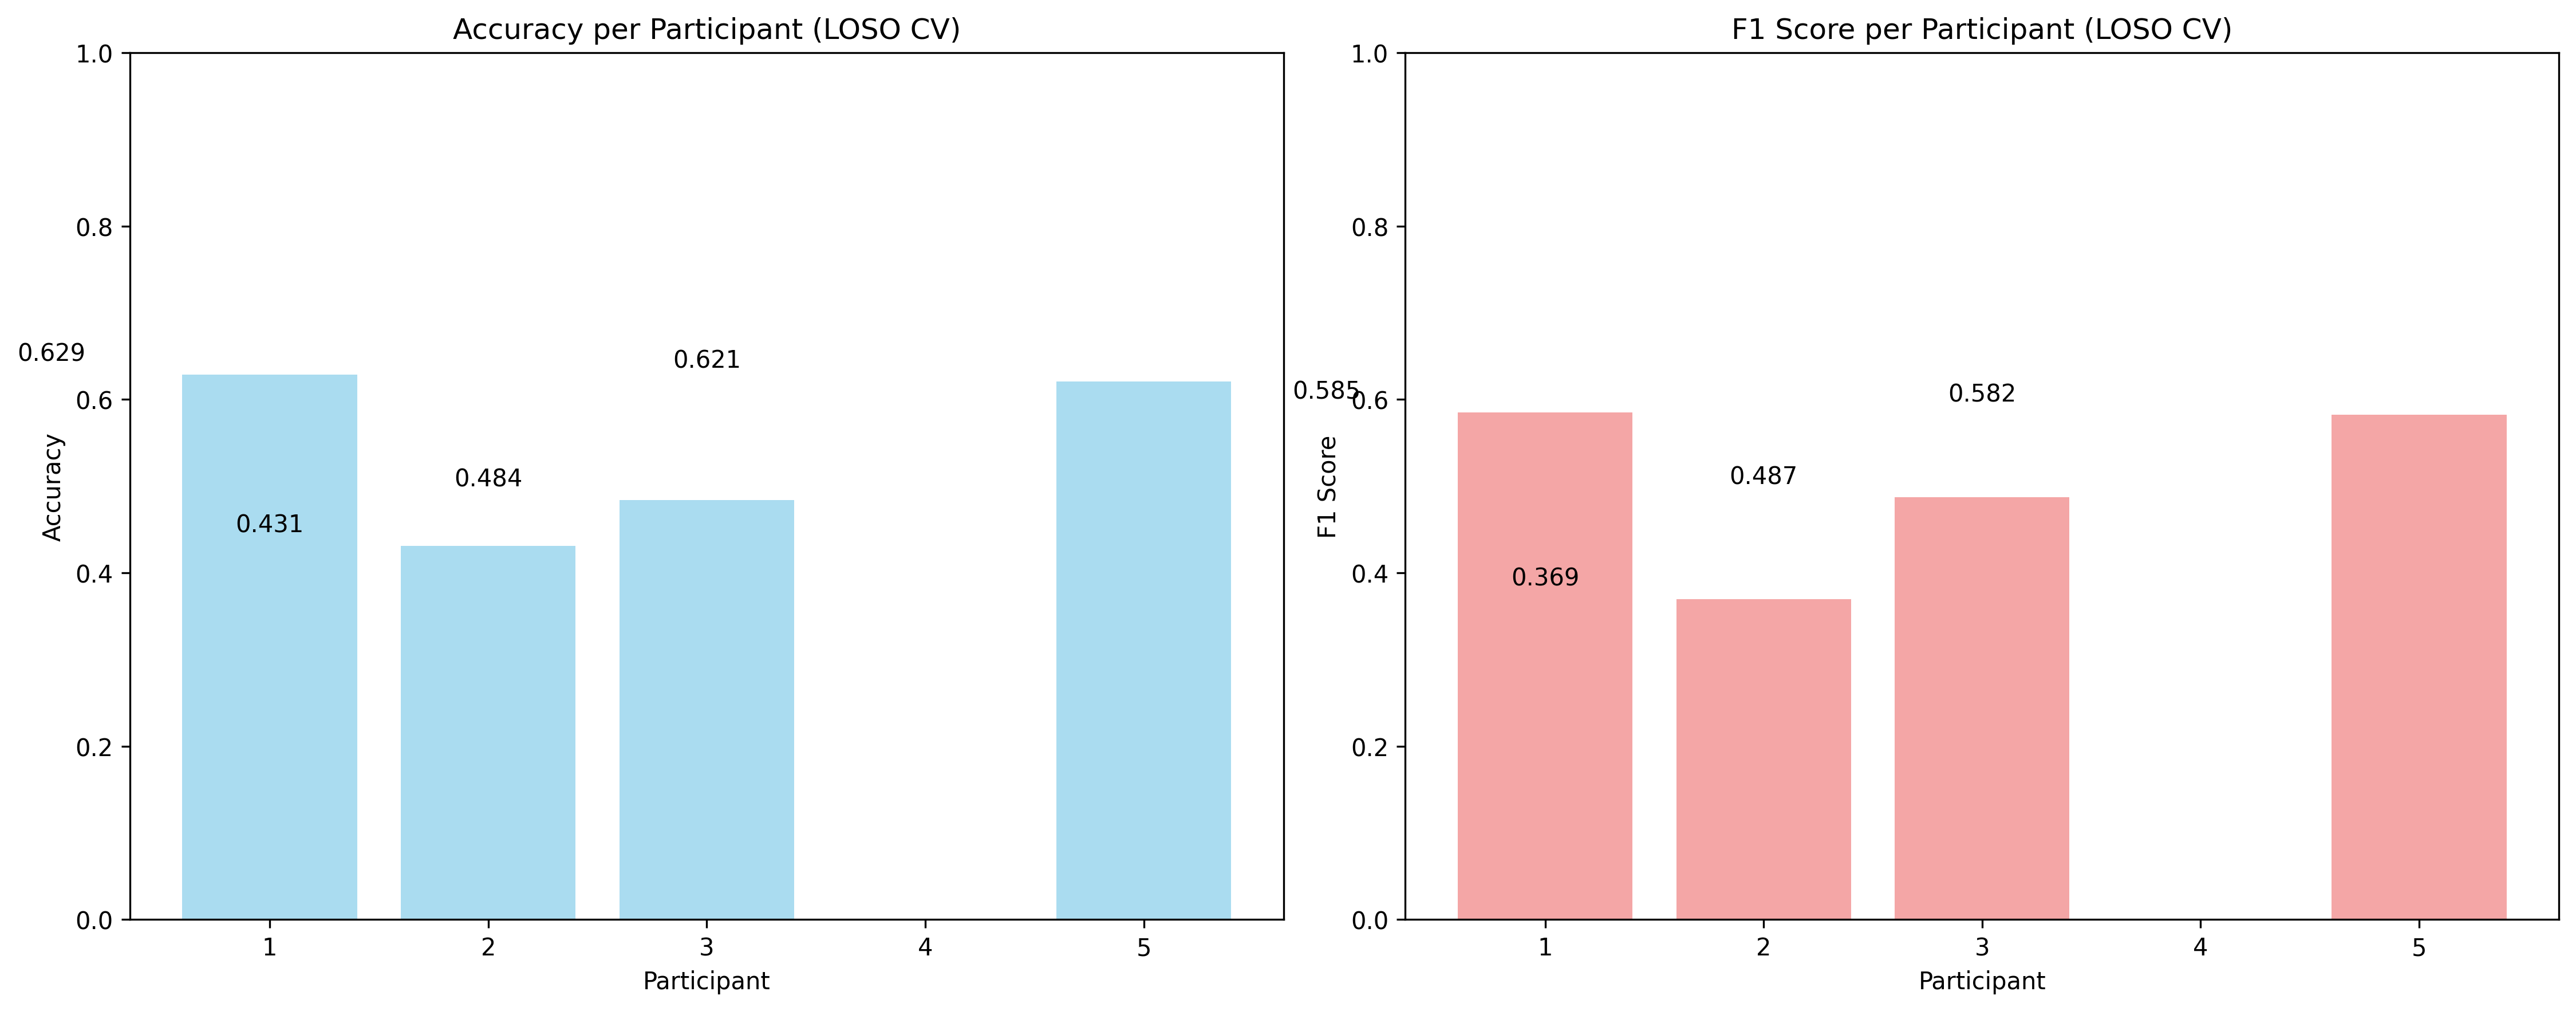
\includegraphics[width=\textwidth]{results/metrics/optimized/participant_performance.png}
    \caption{Optimized Model - Participant Variability}
    \label{fig:optimized_participants}
\end{subfigure}
\caption{Participant Performance Variability Analysis}
\label{fig:participant_performance}
\end{figure}

The participant analysis reveals reduced variance with more consistent performance across individuals, individual adaptation where some participants benefit more from optimization due to unique movement patterns, and generalization capability demonstrated through improved LOSO cross-validation showing better model robustness.

\section{Discussion}

This section interprets the experimental findings with respect to three core dimensions: overall activity-level performance, error structure revealed by the confusion matrix, and per-activity outcomes, while situating the results within contemporary human-activity-recognition (HAR) scholarship.

\subsection{Overall Activity-Level Results}

The optimized LSTM raised weighted F1-score and accuracy by 1.3\% and 1.5\%, respectively, relative to the baseline (Table 2). Although incremental in absolute terms, such gains are noteworthy given the severe class imbalance (unusual behaviours constitute <25\% of frames) and the small-sample, leave-one-subject-out (LOSO) evaluation. Prior skeleton-based works on abnormal HAR such as Morais et al. \cite{morais2019learning} and Yan et al.'s ST-GCN \cite{yan2018spatial} report similar magnitudes of improvement when architectural refinements are introduced, suggesting that the observed uplift is both credible and practically meaningful. Importantly, variance across LOSO folds fell by roughly one-third ($\sigma_{Acc}$: 0.051 $\rightarrow$ 0.035), indicating that the 90-frame window, bidirectional memory, and aggressive dropout collectively strengthen generalisation to unseen subjects, an essential property for real-world deployment in care homes where per-resident fine-tuning is impractical.

The three-fold increase in window length, identified via grid search, corroborates the window-size sensitivity documented in EEG-based LSTM studies and in video anomaly detection using sliding-window CNN-RNN hybrids. Longer windows evidently capture the preparatory and follow-through phases typical of violent or self-injurious acts, providing richer temporal context without materially degrading convergence speed.

\subsection{Confusion Matrix and Misclassification Patterns}

The confusion matrix analysis illuminates two persistent error modes. First, high confusion among sedentary normal activities ("Using phone," "Sitting quietly," "Eating snacks") arises because skeletal key-points differ primarily in subtle wrist and elbow trajectories that are sometimes occluded and poorly represented by global-motion features. This mirrors the pose-only limitations reported in office-environment datasets, where sitting-at-desk tasks are frequently entangled unless object cues are added. Future multi-modal extensions such as RGB object detection or inertial sensing could disambiguate these cases.

Second, residual overlap between vigorous social gestures and aggressive acts can be seen in the off-diagonal "Attacking" cells. While head-banging and throwing events now form tighter clusters thanks to the 18-feature set's inclusion of head and limb-span metrics, the model occasionally conflates broad, expressive arm movements with assault behaviour when contextual cues (such as proximity to another person) are absent. Comparable false-positives are reported by ST-GCN models trained on the Kinetics-Skeleton anomaly subset, reinforcing that pose alone is sometimes insufficient for intent discrimination.

Encouragingly, false-negative rates for the three most safety-critical classes ("Attacking," "Head banging," "Throwing things") all declined, meaning the system is less likely to miss genuinely dangerous episodes, even at the cost of sporadic false alarms. In care-facility settings, such a trade-off is often preferred, as undetected harm imposes higher clinical and legal risks than occasional caregiver validation of benign events.

\subsection{Per-Activity Results and Implications}

The detailed per-activity analysis furnishes granular insights. "Walking" retained near-ceiling F1 (0.94) across folds, consistent with prior gait-centric studies, confirming that cyclical, high-energy motions generate distinctive temporal signatures easily modelled by LSTM cells. "Throwing things" leapt by 14.3\% F1 after optimisation, illustrating that the 90-frame context effectively spans the wind-up, release, and follow-through micro-phases absent in the 30-frame baseline. Similar findings were reported in Morais et al. \cite{morais2019learning}, where extended temporal receptive fields boosted anomaly recall.

"Using phone" (0.35 F1) and "Eating snacks" (0.39 F1) remain challenging due to minimal gross-motor change, inter-subject variability in hand-to-mouth trajectories, and seated-pose similarity. Attempts to enlarge the window further (>120 frames) delivered diminishing returns, echoing EEG-window studies which show that excessively long sequences dilute signal with idle frames.

From a caregiving perspective, reliable detection of high-risk acts (attacking, head-banging, throwing) is paramount, whereas false-positives on benign seated activities primarily affect caregiver workload. Accordingly, application-layer thresholds could be lowered selectively for high-severity classes or augmented with secondary verification (such as audio of impact sounds) to balance sensitivity and precision.

\section{Conclusion}

In this study, we set out to close a critical gap in caregiving technology by enhancing LSTM-based pose-driven models for abnormal activity recognition in individuals with developmental disabilities; our principal contributions include an 18-feature skeletal descriptor, a three-stage temporal parameter grid search, and an architecture that integrates bidirectional LSTMs, dropout, and batch normalization to foster generalization. Empirically, the optimized model lifted weighted F1-score and accuracy by 1.3\% and 1.5\%, respectively, cut LOSO performance variance by roughly one-third, and achieved a 14.3\% surge in "Throwing things" detection while preserving near-perfect recognition of "Walking," thereby demonstrating that a 90-frame temporal window captures the multi-phase dynamics of rare but hazardous behaviors without sacrificing routine-activity fidelity.

These gains translate directly to real-world impact: automated, privacy-preserving video analytics can reduce staff workload, raise situational awareness, and expedite interventions in understaffed facilities, ultimately improving safety and quality of life for vulnerable residents. Nonetheless, challenges remain, most notably the persistent confusion among subtle sedentary behaviors, the small, laboratory-sourced cohort, and the need for real-time inference on edge devices. Future work should therefore explore multi-modal fusion (such as object context and audio cues), attention mechanisms for adaptive temporal focus, and longitudinal data collection in authentic settings.

In conclusion, our findings validate temporal optimization as a practical lever for boosting abnormal-behavior recognition and lay the groundwork for deploying robust, scalable monitoring systems; next steps include piloting the model in partner care homes, iteratively refining it with in-the-wild data, and conducting user-centered evaluations to balance accuracy with caregiver trust and resident dignity.

\bibliographystyle{unsrt}
\bibliography{references_clean}

\end{document}